
There exists a few different frameworks for testing Javascript or
CoffeeScript code. We had previously good experiences from working with
Jasmine\footnote{\url{http://jasmine.github.io/}}. We also found that
this framework seemed to be very popular, actively developed and had
good documentation\footnote{It is worth to mention that the Jasmine
documentation is basically its own test suite with some additional
comments. This works incredibly good in this case, presumably since it
is a test framework and the tests are very well-written.}. Code listing
\ref{lst:jasmine} shows an example of a Jasmine test written in
CoffeeScript. The syntax is inspired by RSpec, which also is an
advantage since RSpec is used for the server side tests.\\

\subsubsection{Test runner}
The Jasmine framework provides a way of writing tests, but a test runner
is also required in order to run the tests. Jasmine ships with a basic
test runner which was used initially, which worked out-of-the box using
the Jasmine Ruby gem. A screenshot of this test runner is shown in
\fref{fig:jasmine_runner}.\\

\begin{figure}
\centering
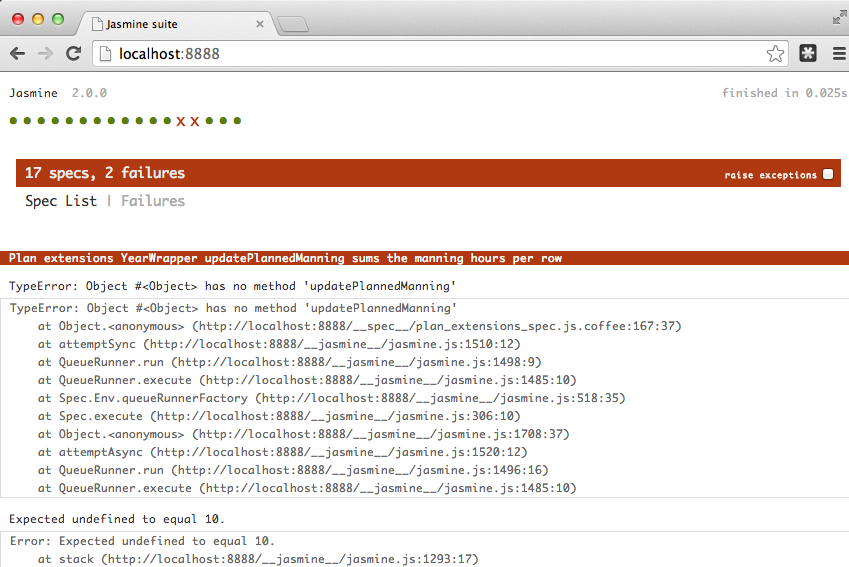
\includegraphics[width=0.8\textwidth]{results/choices/jasmine_runner}
\caption{The test runner bundled with Jasmine.}
\label{fig:jasmine_runner}
\end{figure}

The Jasmine test runner did however have multiple issues. First of all,
it runs completely in the browser. Switching to the browser and reload
the page in order to run the tests are not excessively problematic, but
might be a little bit tiresome in the long run when using a test-driven
development methodology. A larger problem was the fact that the asset
handling, i.e. the compilation of CoffeeScript into Javascript, is
handled by Rails upon each reload. The used version of Rails re-compiles
all assets upon page load if any file has been changed. This process
takes a while, which means that each test run could take up to 10-15
seconds even though the actual tests only takes a fraction of a second
to run. The asset compilation also got stuck for for apparently no
reason once in a while. Since the server port on which the test runner
runs cannot be specified, it is also impossible to restart the test
runner without manually killing its system process.\\

Another issue with the Jasmine test runner is that syntax errors are
printed in the terminal rather than in the browser window where the test
result is reported, which is confusing. In practice, syntax errors was
often undetected for a long time which required more debugging than
necessary.\\

Due to these issues, we switched to the Karma\footnote{
\url{http://karma-runner.github.io/}} test runner. Karma originates from
a master's thesis by \citet{article:karma}, and this covers several
problems with the Jasmine test runner as well as with some other
Javascript test runners. Karma was designed to solve several of these
issues and to be used with test-driven software methodologies. Tests are
run in a browser as soon as a file is changed, and the results are
reported back to the terminal and displayed as shown in
\fref{fig:karma_runner}. Re-compilation of source files and tests is
very fast and we did not experience any stability issues. One minor
drawback is however that pending tests are not displayed very clearly.\\

It took some effort with getting Karma to work with Rails, since it is
written in Node.js and does not have any knowledge about which
CoffeeScript files that exists in the Rails application. The task of
finding the location of all such files became more complex since
external Javascript libraries such as jQuery was loaded as Ruby gems,
and therefore not even located inside the project folder. We ended up
using a slightly modified version of a Rake script from a blog entry by
\citet{web:saunier_angular} for bootstrapping Karma in a Rails
environment. This script basically collects a list of filenames for all
Javascript assets by using Rails internal modules for asset handling,
and injects it into Karma's configuration file.\\

After the case study, we discovered another Javascript test runner
called Teaspoon\footnote{\url{https://github.com/modeset/teaspoon}},
which is built for Rails and can discover assets by default. We believe
that this test runner looks very promising and may be more suitable for
Rails projects than Karma. At the time of this writing, Teaspoon does
not have support for the most recent version of Jasmine and therefore
does not work with our test suite. We were thus unable to evaluate this
test runner any further.\\

\begin{lstlisting}[caption=Example of Jasmine tests for a module (compare with code listing \ref{lst:rspec}).,
                   label=lst:jasmine, float=t, language=HTML]
describe 'Math', ->
  describe 'minus', ->
    it 'returns the difference between two positive integers', ->
      expect(Math.minus(3, 1)).toEqual(2)

    it 'returns the sum if the second integer is negative', ->
      expect(Math.minus(5, -2)).toEqual(7)

  describe 'plus', ->
    it 'returns the sum of two positive integers', ->
      expect(Math.plus(1, 2)).toEqual(3)
\end{lstlisting}

\begin{figure}
\centering
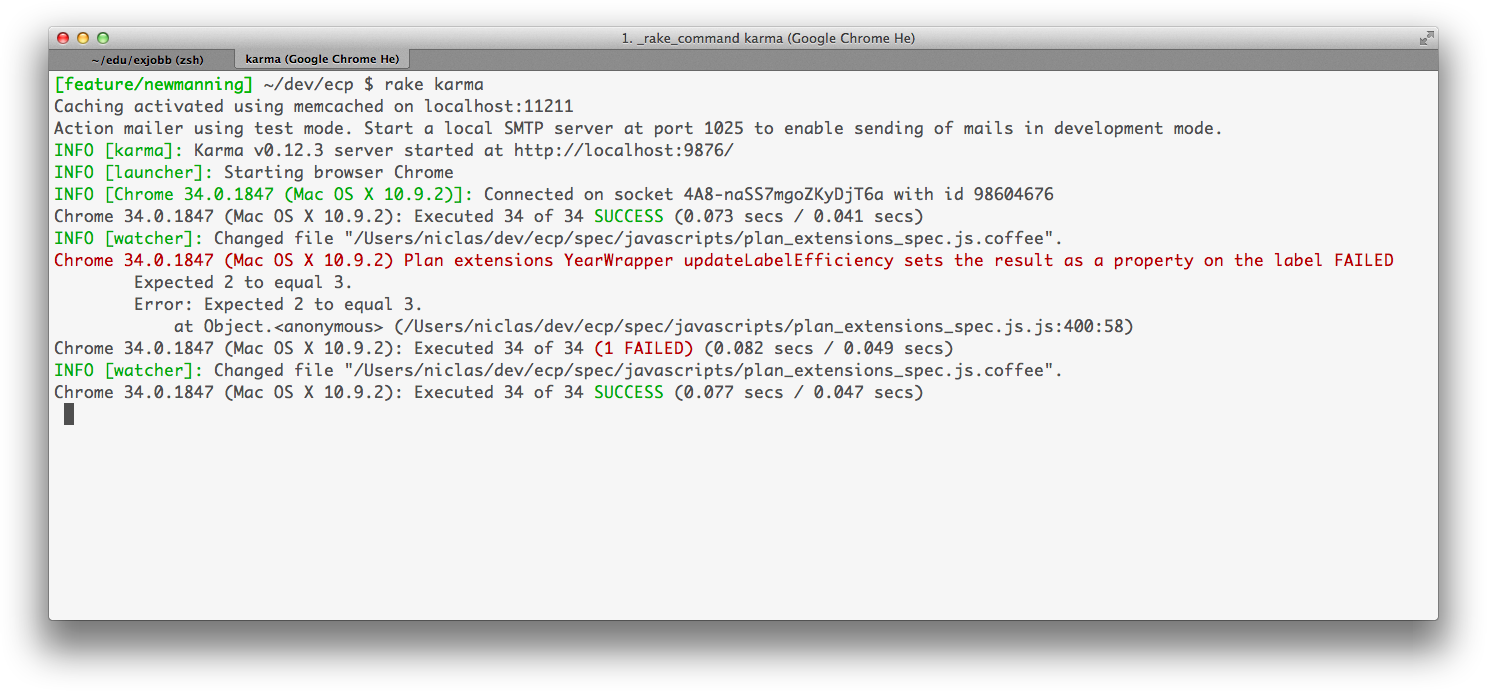
\includegraphics[width=0.8\textwidth]{results/choices/karma_runner}
\caption{The Karma test runner.}
\label{fig:karma_runner}
\end{figure}
